\chapter{Implementatie}
Na de literatuurstudie en de ontwerpfase, is het tijd om het ontwerp dat besproken werd in Hoofdstuk~\vref{sec:anaEnOntwerp} te implementeren.
Als programmeertaal werd Python gekozen zodanig dat de applicatie uniform is met het testraamwerk.
In de komende secties worden de verschillende implementatie beslissingen toegelicht en wordt de geschreven code toegelicht.
De applicatie werd geschreven met twee doelen in het achterhoofd: de demo die gegeven gaat worden tijdens de verdediging en een basis vormen voor Televic om van te vertrekken.
Het doel van de presentatie is het tonen van het installatieproces beginnende bij de creatie van een installer tot het installeren zelf in een container in een field dock.
Om dit te kunnen realiseren, was het niet nodig/mogelijk om alle nodige functionaliteiten te implementeren en toe te voegen aan de applicatie.
Tijdens het implementeren, werden de server-side en client-side van elkaar gescheiden en er werden twee verschillende packages aangemaakt.
In wat volgt, zullen deze dan ook afzonderlijk besproken worden.

\section{Server-side}
\paragraph{Initialisatie} 
De server package bevat alle logica die hoort bij het release dock als bij de broker, maar bevat ook enkele modules die gebruikt worden om de realiteit af te beelden.
De flow van de applicatie begint met het opstarten van de deployment\_server module.
Deze module zal een release dock, een broker en een packager opstarten.
Vervolgens wordt het release dock gesubscribed voor de berichten van het type new, change en rapport.
Nadat de nodige services zijn opgestart, is het release dock klaar voor het afhandelen van alle nodige taken zoals het afhandelen van binnenkomende berichten.

Zowel het release dock als de broker erven eigenschappen van de klasse Dock.
Dit is zichtbaar in Figuur~\vref{fig:classDock}.
Aangezien alle docks en de broker dezelfde functionaliteiten moeten hebben (openen van een socket, luisteren voor data op de socket, versturen van berichten en afhandelen van berichten), is het eenvoudig om deze functionaliteiten in de superklasse te steken.
Een soortgelijke strategie wordt toegepast voor de agenten aangezien elk type van agent een actie moet kunnen uitvoeren.
De nodige methodes worden vervolgens ingevuld in de subklasse. 

\begin{figure}[!ht]
\centering
\makebox[0pt]{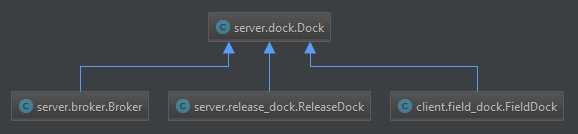
\includegraphics[scale=0.7]{afbeelding/classDock.png}}
\caption{Klassendiagram van Dock}
\label{fig:classDock}
\end{figure}

\paragraph{Grafische User Interfaces}
Het is ook mogelijk om de Grafische User Interface (GUI) op te starten door middel van de ``Enter'' toets.
Vanuit de GUI is het mogelijk om de verschillende clients te controleren en is het mogelijk om nieuwe installers te creëren.
De GUI werd gemaakt met de Python bibliotheek wxPython\footnote{\url{https://wxpython.org/}} en met de hulp van wxFormBuilder\footnote{\url{https://github.com/wxFormBuilder/wxFormBuilder}} werd basis code gegenereerd.
De nodige methodes werden vervolgens overschreven in de module overview\_impl.
Via deze methode wordt een gelijkaardig resultaat behaald voor het maken van de GUI voor de installer creatie.

\paragraph{Berichten versturen}
Bij het versturen van een bericht moet eerst een object aangemaakt worden van de Message klasse.
Vervolgens wordt de inhoud toegevoegd aan het bericht en kan het verzonden worden naar de broker.
In de broker wordt gecontroleerd welk type bericht het is om het dan vervolgens door te sturen naar alle doelen die in de gepaste list zitten.
Voordat het bericht wordt doorgestuurd wordt het eerst ingepakt in een ander bericht met als type notificatie.
Zo weet de ontvanger dat het bericht afkomstig is van de broker en is weet de ontvanger dat het data veld het doorgestuurde bericht bevat.
Deze kan vervolgens uitgepakt worden.
Afhankelijk van het type van het doorgestuurde bericht zal de correcte methode opgeroepen worden.

\paragraph{Installer creatie}
In de overzicht GUI is het mogelijk om een nieuwe installer te maken.
Met behulp van de aparte GUI, die geïmplementeerd wordt door de module release\_creator\_impl, is het mogelijk om een installer te definiëren.
Tijdens het samenstellen van de installer kunnen verscheidene nieuwe pakketten aangemaakt worden door de bovenste velden meermaals in te vullen.
Hierbij is het belangrijk om te weten dat een folder moet geselecteerd worden als bestandslocatie.
Alle bestanden aanwezig in de geselecteerde folder worden tijdens de creatie verplaatst naar de correcte locatie.
Bij het invullen van de gegevens van de installer moet ook een folder geselecteerd worden waarin de installer moet terecht komen.

Bij het indienen van de gegevens van de installer zelf worden de nodige handelingen uitgevoerd om een correcte installer te produceren.
Eerst worden de pakketten en installer toegevoegd aan de databank.
Vervolgens wordt de nodige folder structuur opgebouwd zoals aangegeven werd in Figuur~\vref{fig:installerStructuur}.
In de config folder wordt een leeg Dockerfile en een metadata bestand met daarin de volledige beschrijving van de installer.
Vervolgens wordt gecontroleerd 

\section{Client-side}